\documentclass[../main.tex]{subfiles}
\graphicspath{{img},{img/ink},{ink}}

\begin{document}

\begin{tcolorbox}[
    width=\textwidth,
    height=\textheight,
    title=Phyphox: Magnetfeld der Erde,
    fonttitle=\Large,
    before title=\vspace{0.2cm}, after title=\vspace{0.2cm},
    colback=white,
    title filled=true, 
    colbacktitle=myorange,
    colframe=black,
    coltitle=black,
    ]


    \begin{minipage}[]{0.8\textwidth}

        \textbf{Klassenstufe}: 9/10

        \vspace{0.5cm}

        \textbf{Fachlicher Bezug}: Erdmagnetfeld, Inklination, Inklinationskarte

        \vspace{0.2cm}
        \textbf{Material}: 
        \begin{itemize}[noitemsep]
            \item Geodreieck
            \item Lot
            \item Halterung
            \item Handy + Phyphox
        \end{itemize}


    \end{minipage}
    \hspace{0.3cm}
    \begin{minipage}[]{0.15\textwidth}
        \vspace{0.3cm}
        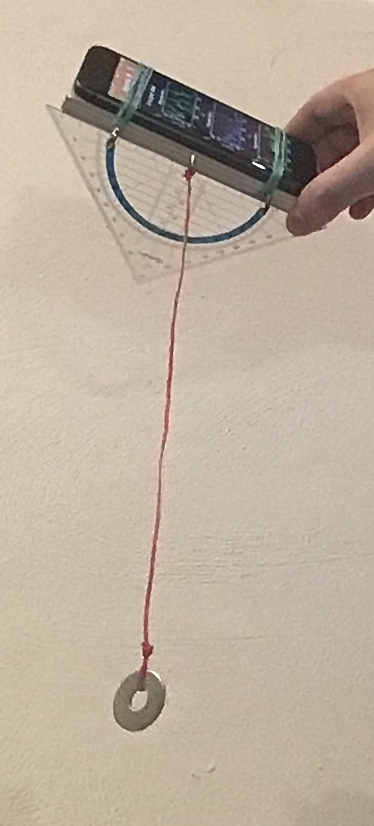
\includegraphics[width=\textwidth]{img/versuchsaufbau}
    \end{minipage}

    \vspace{0.2cm}
    \begin{minipage}[]{0.75\textwidth}
        \textbf{Aufbau}: In der Phyphox-App wird unter dem Reiter \glqq Sensoren\grqq{} die Auswahl \glqq Magnetfeld\grqq{} getroffen. Im Experiment werden dann die Graphen für x,y und z-Richtung des Magnetfelds angezeigt. Das Handy wird in der Halterung fixiert. Lot und Geodreick werden seitlich angebracht.  

        \vspace{0.5cm}
        \textbf{Durchführung}: Das Handy wird ausgerichtet, sodass x- und y-Richtung des Magnetsensors einen Wert von $0$ anzeigen. Der Wert des Magnetfelds in z-Richtung wird notiert. Der Winkel, den das Lot am Geodreicke anzeigt, wird abgelesen.  
    \end{minipage}
    \hspace{0.3cm}
    \begin{minipage}[]{0.2\textwidth}
        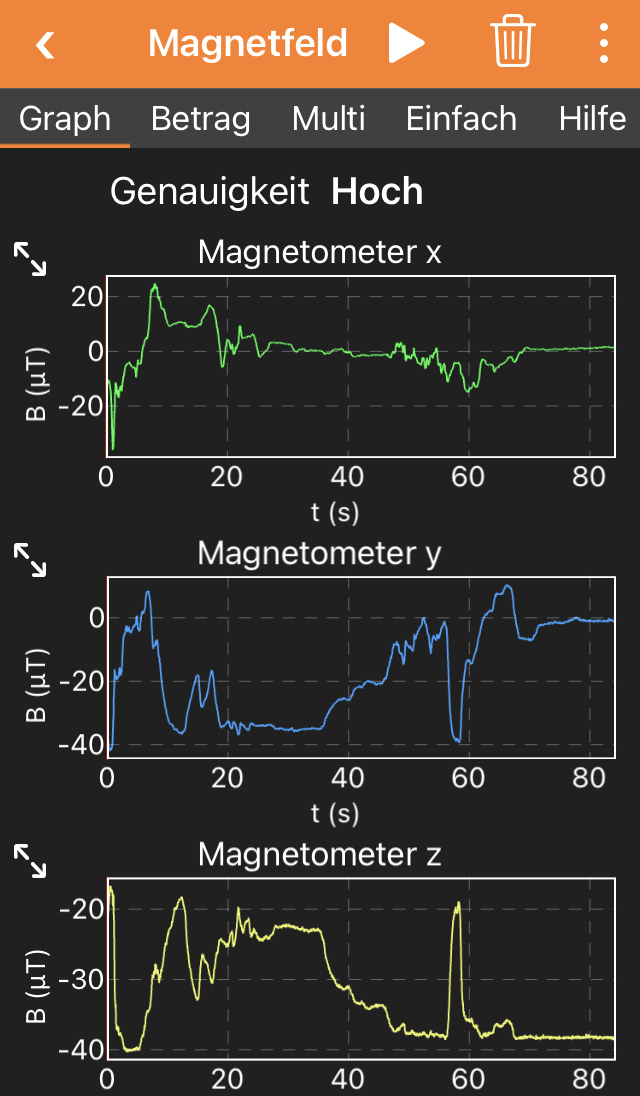
\includegraphics[width=\textwidth]{img/app}
    \end{minipage}

    \vspace{0.5cm}
    \textbf{Ergebnis}: 
    Der Winkel des Lots am Geodreick entspricht dem Inklinationswinkel $i$. In Deutschland erhält man einen Wert zwischen $60^{\circ}$ und $70^{\circ}$. Die z-Richtung des Magnetsensors liefert die Stärke des Magnetfelds. Man erhält Werte im Bereich von $B=40-50\, \mu$T. \\
    Das \glqq World Magnetic Model\grqq{} (https://www.ncei.noaa.gov/products/world-magnetic-model) liefert offizielle Daten um diese Messwerte nachzuprüfen. Inklination $I$ (Karte mitte) und Stärke $F$ (Karte rechts) des Magnetfelds liegen als Karten vor.

    \vspace{0.5cm}
    \begin{center}
        \begin{minipage}[]{0.26\textwidth}
            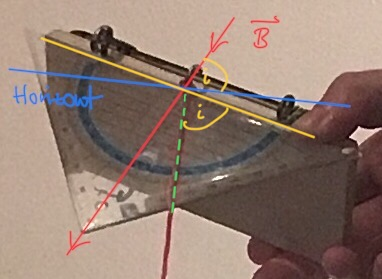
\includegraphics[width=\textwidth]{img/inklination}  
        \end{minipage}
        \hspace{0.15cm}
        \begin{minipage}[]{0.3\textwidth}
            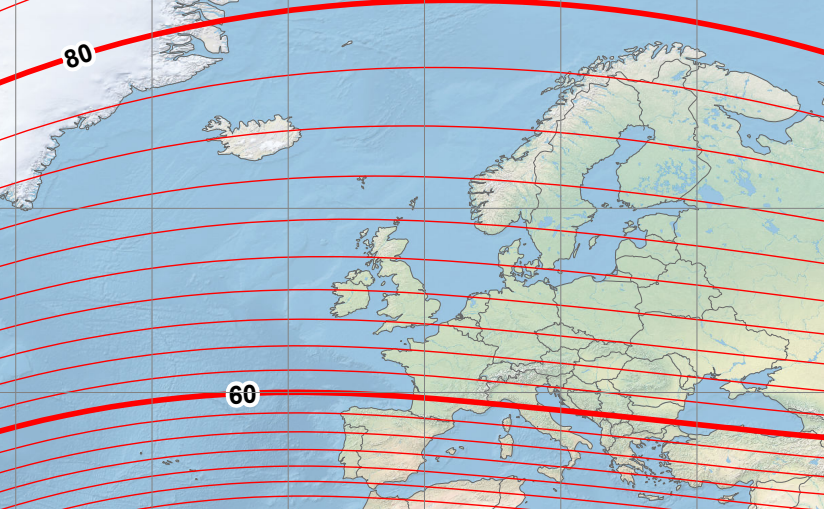
\includegraphics[width=\textwidth]{img/inklinationskarte}
        \end{minipage}
        \hspace{0.15cm}
        \begin{minipage}[]{0.33\textwidth}
            \includegraphics[width=\textwidth]{img/stärke}
        \end{minipage}
    \end{center}

\vspace{0.5cm}
    \textbf{Bemerkung}: Um eine sinnvolle Messung durchzuführen, ist es notwendig sich von Gebäuden, Autos oder metallischen Strukturen fernzuhalten. Auch die Handyhülle sollte bei einem magnetischen Verschluss entfernt werden.\\
    \begin{minipage}[]{0.85\textwidth}
            Als Ersatz für Geodreieck und Lot kann auch ein eigenes Experiment erstellt werden, in dem die Neigung des Handys über die Beschleunigungssensoren berechnet wird.
  
        \end{minipage}
        \hspace{0.3cm}
        \begin{minipage}[]{0.1\textwidth}
            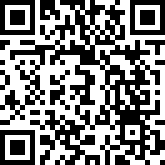
\includegraphics[width=\textwidth]{img/qr_code}
        \end{minipage}

    
\end{tcolorbox}


\end{document}
